\documentclass{article}
\usepackage{amsmath}
\usepackage{graphicx}
\usepackage{biblatex} 
\usepackage{authblk}
\usepackage{mathtools}
\usepackage{hyperref}
\addbibresource{three_books.bib}

\title{Gaussian processes and their equivalent Bayesian linear regressions}
\author[1]{Douglas Mason}
\affil[1]{Koyote Science, LLC \footnote{\href{http://www.koyotescience.com}{\texttt{http://www.koyotescience.com}}}}
\date{September 2021}

\begin{document}

\maketitle

\section{Introduction}

Finding the equivalent Bayesian linear regression (BLR) to a Gaussian process (GP) can provide substantial benefits in modeling including (1) enormous efficiency savings with large amounts of data, (2) access to incremental (sequential or online) computation methods, (3) access to vetted approximation methods for efficiency (such as the Laplace approximation for regressors, not just classifiers), (4) easier interpretability, and (5) the ability to effortlessly to combine multiple models into one without using bespoke software libraries. However, while the three major textbooks on the subject \cite{bishop, murphy, rasmussen} cover the subject extensively, it surprised me that they didn't provide a practical side-by-side comparison or recipe for converting the kernel used to generate a GP to an equivalent set of basis functions for a BLR. Moreover, we can look at Gaussian processes as an extension of Bayesian linear regression into the territory of small data, where the number of training points is less than the number of features, which is an important problem space for optimization procedures where evaluating a function may take a substantial amount of time. Bringing together the best of both worlds is enormously beneficial to anyone working within the optimization problem space.

Why this subject isn't lucidly explained in any established textbooks or lectures notes we could find remains a mystery to me, but it actually takes a lot of work to get the equivalence just right. This document covers the recipe we arrived at after working through the problem, and the insights we learned along the way. You are free to explore for yourself using the  Github repository which can be accessed at https://github.com/KoyoteScience/GP-BLR.

Studying BLR and GP side-by-side is critical for developing any Bayesian application, since these are among only a few models in  circulation that allow you to learn the parameters using explicit and deterministic update rules. In other words, if we want to put Bayesian models into production with calibrated uncertainty predictions, these two are the robust, reliable baselines from which all other approaches are compared. Moreover, because the computation of these models is deterministic, we avoid the horrible pitfalls of Markov chain Monte Carlo, and because they are exact, we avoid the pitfalls of variational inference. As we will cover, both are actually parts of the same continuum between high featurization and large amounts of data. 

A quick glossary: scalars are presented as upper- or lower-case English or Greek letters with normal weight, such as $n$ or $N$, while vectors are presented as lower-case English or Greek letters in bold, such as $\mathbf{v}$ or $\boldsymbol{\phi}$. Row vectors are presented normally, and column vectors with the transpose operator $\mathbf{v}^\top$. The dot or inner product is two vectors multiplied as $\mathbf{v}^\top \mathbf{v}$ and the outer product is two vectors multiplied as $\mathbf{v} \mathbf{v}^\top$. Matrices are presented as upper-case letters with bold weight, such as $\mathbf{M}$ or $\boldsymbol{\Phi}$. For variables that refer to the posterior (after $N$ training samples), their prior counterparts are denoted by the $p$ subscript.

\section{Bayesian linear regression}

Bayesian linear regression can be defined by modeling a predictor
\begin{equation}
    y=f(\mathbf{x})=\boldsymbol{\theta}^\top\mathbf{x}
\end{equation} 
given a prior distribution for our model parameters $\boldsymbol{\theta}$ defined as 
\begin{equation}
    \boldsymbol{\theta}_p \sim \mathcal{N}(\mathbf{0},\Sigma_p)
\end{equation} 
using the convention whereby the normal distribution is defined by two arguments, the means in each dimension and the covariance among the dimensions. Given a set of $N$ observations, over the independent space $\mathcal{X}$ and the dependent space $\mathcal{Y}$, gives us the matrix $\mathbf{X}$ of observations in the independent space and the vector $\mathbf{y}$ of corresponding observations in the dependent space.
\begin{equation}
    \boldsymbol{\Sigma}^{-1} = \sigma^{-2}\mathbf{XX}^\top + \boldsymbol{\Sigma}_p^{-1}
\end{equation}

This gives us
\begin{equation}
    \boldsymbol{\theta}\sim\mathcal{N}( \sigma^{-2}\boldsymbol{\Sigma} \mathbf{X}^\top \mathbf{y},\boldsymbol{\Sigma})
\end{equation} 
and
\begin{equation}
    \mathbf{y}\sim\mathcal{N}\left(\sigma^{-2}\mathbf{X}  \boldsymbol{\Sigma} \mathbf{X}^\top \mathbf{y} ,\mathbf{X}^\top \boldsymbol{\Sigma} \mathbf{X} +\sigma^2\ \mathbf{I}_N\right)
\end{equation} 
where $\sigma$ is the noise parameter, or the square-root of the sum of squared residuals., and the term $\sigma^2 \mathbf{I}$ provides the uncertainty for repeated measurements of $y$ at the same $\mathbf{x}$.

The equivalent perspective of $L2$ regularization gives us a regularization constant \begin{equation}\label{eq:lambda}\lambda=\sigma^2/\sigma_p^2\end{equation} where $\sigma_p$ represents the noise term for the prior. This implies that we more strongly regularize our results (draw weights towards zero) as we decrease the noise parameter in the prior compared to the noise parameter in the posterior. 

The above formulation makes it clear how the covariance matrix of our parameters evolves over inference from $\boldsymbol{\Sigma}_p$ to $\boldsymbol{\Sigma}$ and how this affects our predictions. If we don't keep $\sigma$ fixed but instead learn it from our data or use linear algebra identities to define it, we may prefer to work with the quantity 
\begin{equation}
\label{eq:S}
    \mathbf{S}^{-1} = \sigma^2\boldsymbol{\Sigma}^{-1}=\mathbf{XX}^\top + \sigma^2\mathbf{S}_p^{-1}
\end{equation}
giving us
\begin{equation}
    \boldsymbol{\theta}\sim\mathcal{N}( \mathbf{S} \mathbf{X}^\top \mathbf{y},\sigma^2\mathbf{S})
\end{equation} 
and
\begin{equation}
    \mathbf{y}\sim\mathcal{N}\left(\mathbf{X}  \mathbf{S} \mathbf{X}^\top \mathbf{y} ,\sigma^2\left(\mathbf{X}^\top \mathbf{S}\mathbf{X} + \mathbf{I}_N\right)\right)
\end{equation}
which makes it far clearer that the covariance matrices for both our weights and predictions are proportional to the noise parameter squared, while the mean weights and predictions only depend upon it through Equation \ref{eq:S}. This formulation also makes the connection to kernels in Gaussian processes clearer in later sections.


\section{Bayesian linear regression with basis functions}

We now transform our independent space using a set of basis function $\boldsymbol{\phi}(\mathbf{x})$ and assume that
\begin{equation}
    y_\ast=f(\mathbf{x_\ast})=\boldsymbol{\theta}^\top\boldsymbol{\phi}(\mathbf{x_\ast})
\end{equation} 
Given $N$ training samples, $N_\ast$ test samples, and an $N_B$-dimensional basis vector, we arrive at the notation $\Phi=[\boldsymbol{\phi}(\mathbf{x}_0),\boldsymbol{\phi}(\mathbf{x}_1),\dots,\boldsymbol{\phi}(\mathbf{x}_{N}))]^\top$, which is a $N \times N_B$ matrix, and  $\boldsymbol{\phi}_\ast=\boldsymbol{\phi}(\mathbf{x}_\ast)$, which is a $N_\ast \times N_B$ matrix. This gives us the covariance function:
\begin{equation}
\label{covariance_matrix}
    \boldsymbol{\Sigma}^{-1} = \sigma^{-2} \boldsymbol{\Phi}  \boldsymbol{\Phi}^\top +  \boldsymbol{\Sigma}_p^{-1}
\end{equation} 
where we note that the calculation in involves matrix multiplications on the scale $N_B \times (N \times N) \times N_B + N_B \times N_B$. In other words, we perform a summation (integration or dot product) over the training data points.

Similarly,
\begin{equation}
\label{theta_distribution}
    \boldsymbol{\theta}\sim\mathcal{N}( \sigma^{-2}\boldsymbol{\Sigma} \boldsymbol{\Phi}^\top \mathbf{y},\boldsymbol{\Sigma})
\end{equation} 
involves matrix multiplications on the scale $N_B \times (N_B \times N_B) \times (N \times N)$ for the mean, that is, we perform a summation over the basis vector and the training data. We now have model parameters for each $N_B$ dimension in the basis functions. This gives us
\begin{equation}
\label{BLR_posterior}
    \mathbf{y}(\mathbf{x})\sim\mathcal{N}\left(\sigma^{-2}\boldsymbol{\Phi}  \boldsymbol{\Sigma} \boldsymbol{\Phi}^\top\mathbf{y} ,\boldsymbol{\Phi}^\top\boldsymbol{\Sigma}\boldsymbol{\Phi}+\sigma^2 \mathbf{I}_N\right)
\end{equation} 
and
\begin{equation}
\label{BLR_posterior}
    y_\ast(\mathbf{x}_\ast)\sim\mathcal{N}\left(\sigma^{-2}\boldsymbol{\phi}_\ast  \boldsymbol{\Sigma} \boldsymbol{\Phi}^\top\mathbf{y} ,\boldsymbol{\phi}^\top_\ast \boldsymbol{\Sigma}\boldsymbol{\phi}_\ast+ \sigma^2\right)
\end{equation} 
with the associated matrix multiplications on the scale $N_\ast \times(N_B \times N_B) \times (N_B \times N_B) \times (N \times N)$ for the mean and $N_\ast \times (N_B \times N_B) \times (N_B \times N_B) \times N_\ast$ for the covariance. In other words, we most of our summations are over the basis dimensionality $N_B$ and some over the training set dimensionality $N$. An example Bayesian linear regression can be seen in Figures  \ref{fig:priors_and_posteriors} \ref{fig:example_regression}.

Note that for fixed $\sigma$ and $\sigma_p$, we set our prior parameters $\boldsymbol{\theta}=\mathbf{0}$ to zero and the covariance matrix of those parameters $\boldsymbol{\Sigma}_p=\frac{\sigma_p^2}{\sigma^2}\mathbf{I}_{N_B}$. In other words, our model parameters are uncorrelated with a mean of zero, which can be seen by the flat prior mean and predictive uncertainty in Figure \ref{fig:example_regression}. When we sample our model parameters for the posterior, however, the covariance matrix will exhibit off-diagonal entries that correlate the model parameters with each other due to the fact that basis functions overlap. This added correlation is not required to generate smooth samples of our prediction distribution. As can be seen in Figure \ref{fig:priors_and_posteriors}, our priors are just as smooth as our posteriors, even though if we were to plot the centers of each basis function multiplied by their weights, the prior would be a random noise plot and the posterior would be smooth. The reason the priors are still smooth despite having a diagonal covariance matrix is that the random fluctuations of the parameters add up over the extended basis functions to produce a smooth sum.

Meanwhile, the alternative formulation gives us 
\begin{equation}
\label{eq:define_S}
    \mathbf{S}^{-1} = \sigma^2\boldsymbol{\Sigma}^{-1}=\boldsymbol{\Phi \Phi}^\top + \sigma^2\mathbf{S}_p^{-1}
\end{equation}
\begin{equation}
\label{theta_distribution}
    \boldsymbol{\theta}\sim\mathcal{N}( \mathbf{S} \boldsymbol{\Phi}^\top \mathbf{y},\sigma^2\mathbf{S})
\end{equation} 
\begin{equation}
\label{BLR_posterior}
    \mathbf{y}(\mathbf{x})\sim\mathcal{N}\left(\boldsymbol{\Phi}  \mathbf{S} \boldsymbol{\Phi}^\top\mathbf{y} ,\sigma^2\left(\boldsymbol{\Phi}^\top\mathbf{S}\boldsymbol{\Phi}+\mathbf{I}_N\right)\right)
\end{equation} 
\begin{equation}
\label{BLR_posterior}
    \mathbf{y_\ast}(\mathbf{x}_\ast)\sim\mathcal{N}\left(\boldsymbol{\phi}_\ast  \mathbf{S} \boldsymbol{\Phi}^\top\mathbf{y} ,\sigma^2\left(\boldsymbol{\phi}^\top_\ast \mathbf{S}\boldsymbol{\phi}_\ast+ \mathbf{I}_{N_\ast}\right)\right)
\end{equation} 

\section{Gaussian processes}

The Gaussian Process (GP) is defined differently. Instead of considering a set of multi-valued basis function vectors defined for each point in independent space $\mathbf{x}$, we consider a single-valued function that takes as two points in the independent space as its arguments. This function is the kernel $k(\mathbf{x},\mathbf{x}')$ which can be extrapolated to multiple observations at once as the matrix $\mathbf{K}(\mathbf{X},\mathbf{X}')$. We thus draw the associated observations in the dependent space $\mathbf{y}$ according to the normal distribution using the prior distribution:
\begin{equation}
    \begin{bmatrix}
    \mathbf{y} \\
    \mathbf{y_\ast}
    \end{bmatrix} \sim
    \mathcal{N}\left(\mathbf{0},
    \begin{bmatrix}
    \mathbf{K}(\mathbf{X},\mathbf{X}) & \mathbf{K}(\mathbf{X},\mathbf{X}_\ast) \\
    \mathbf{K}(\mathbf{X}_\ast,\mathbf{X}) & \mathbf{K}(\mathbf{X}_\ast,\mathbf{X}_\ast)
    \end{bmatrix}\right)
\end{equation} 

Let us simplify this notation a bit:
\begin{equation}
    \begin{bmatrix}
    \mathbf{y} \\
    \mathbf{y_\ast}
    \end{bmatrix} \sim
    \mathcal{N}\left(\mathbf{0},
    \begin{bmatrix}
    \mathbf{K} & \mathbf{K}_\ast \\
    \mathbf{K}^\top_\ast & \mathbf{K}_{\ast\ast}
    \end{bmatrix}\right)
\end{equation} 
This is a distribution over the observations and the new test points (denoted with the asterisk) jointly. What does it looks like from the new test point's perspective after we account for the observations?  We can solve this using Section 4.3.4 and Equation 4.69 in \cite{murphy}, obtaining the posterior distribution:
\begin{equation}
\label{GP_posterior}
\mathbf{y}_\ast\sim\mathcal{N}\left(\mathbf{K}_\ast^\top \mathbf{K}^{-1}\mathbf{y},\mathbf{K}_{\ast\ast}-\mathbf{K}_\ast^\top \mathbf{K}^{-1}\mathbf{K}_\ast \right)
\end{equation}

Note that the Gaussian process formalism presented here assumes that the variance of our targets $\sigma_\mathbf{y}$ is equal to one. However, we can adjust for this by regressing against $\mathbf{y}/\sigma_\mathbf{y}$ and then multiplying our predictions $\sigma_\mathbf{y}$ (and similarly for the prediction standard deviations). Later, we will show that the variance can be tuned by how we normalize our kernel. The calculations for a Gaussian process require summations in the matrix multiplication at the scale of $N_\ast \times (N \times N) \times (N \times N)$ for the mean and $N_ast \times (N \times N) \times (N \times N) \times N_\ast$ for the covariance, thus all summations are over the training set dimensionality $N$ rather than the basis set dimensionality $N_B$, which never appears in the GP. This is the essence of the "kernel trick". An example Gaussian process regression can be seen in Figures  \ref{fig:priors_and_posteriors} \ref{fig:example_regression}.

\begin{figure}
    \begin{center}
    \includegraphics[width=0.75\linewidth]{prior_samples}
    \includegraphics[width=0.75\linewidth]{posterior_samples}
    \caption{The Bayesian linear regression and Gaussian process models both define a distribution of functions that fit our data and which are defined by the hyperparameters of the corresponding model. For the GP, these hyperparameters are the kernel function. For the BLR, these hyperparameters are the basis functions and the ratio $\sigma^2/\sigma_p^2$. Fitting to the data is equivalent to filtering the distribution of prior functions to the distribution of posterior functions, which can be seen by Bayes rule $\text{posterior}\propto\text{likelihood}\times\text{prior}$. At top, we show ten samples of the prior functions, and at bottom, ten samples of the posterior functions for the data show in red sampled from the objective. Figure \ref{fig:example_regression} shows a simplification of the bottom plot, replacing the samples with their mean and two standard deviations. This figure was created with the associated code on Github.}
    \label{fig:priors_and_posteriors}
    \end{center}
\end{figure}

\begin{figure}
    \begin{center}
    \includegraphics[width=0.75\linewidth]{prior_regression_results}
    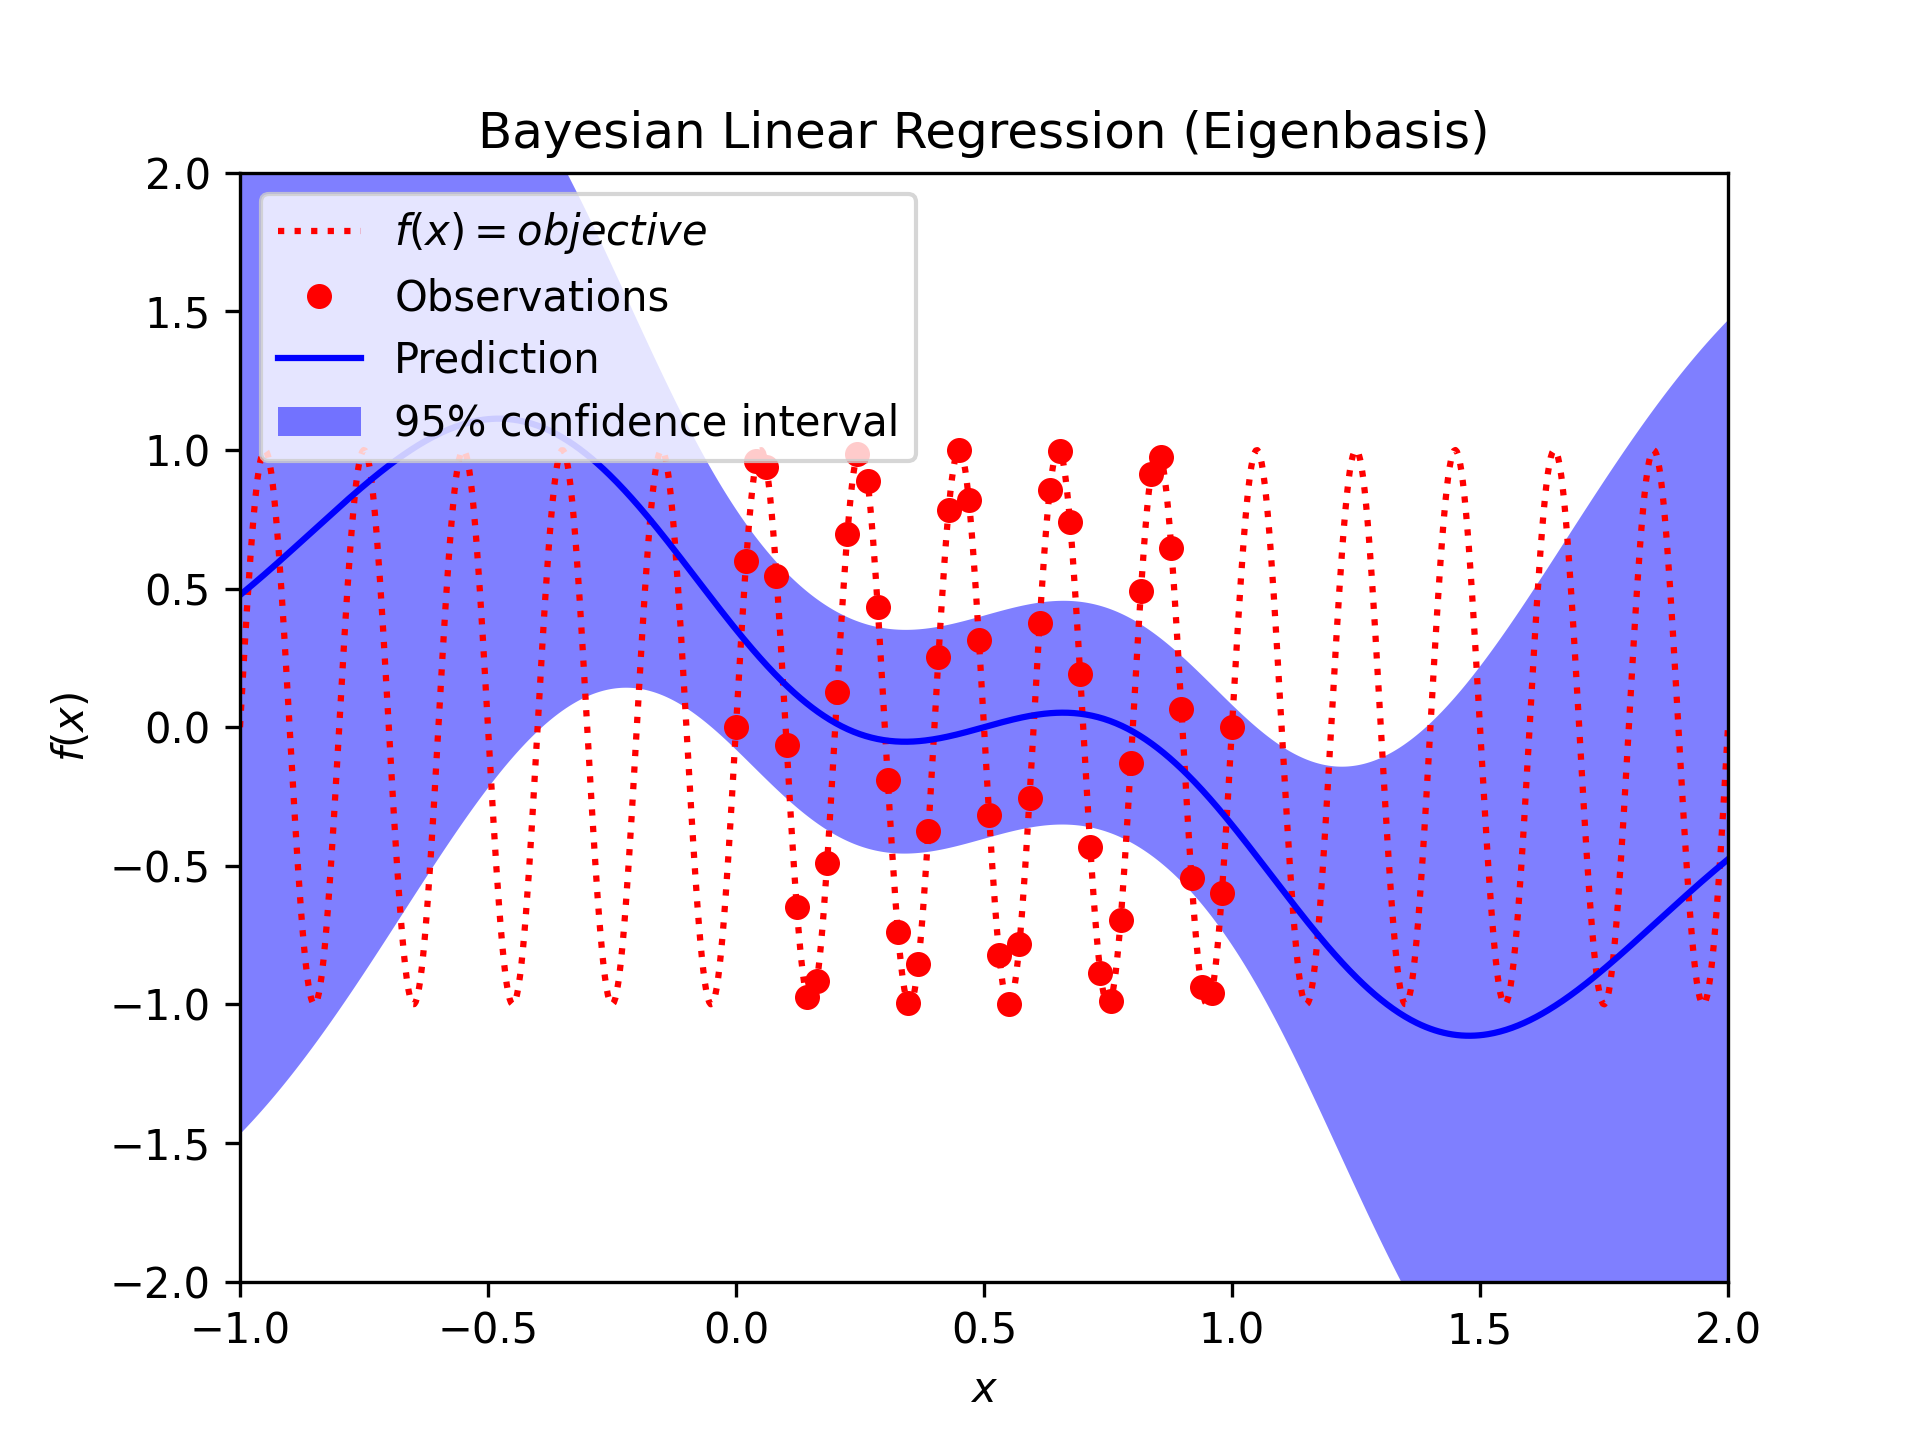
\includegraphics[width=0.75\linewidth]{regression_results}
    \caption{Regression results for all three approaches for an objective function that is a sine wave, matching Figure \ref{fig:priors_and_posteriors} but now showing the mean (blue line) and two standard deviations of the prediction uncertainty (blue area). At top, the prior, and at bottom, the posterior. The wavelength is set to 0.5, a Gaussian kernel with length scale set to 0.5, the noise parameter set to 0.1, with 1000 basis centers spread across a domain from -2 to 3, and 20 training data points spread equidistantly over a domain from 0 to 1. This figure was created with the associated code on Github.}
    \label{fig:example_regression}
    \end{center}
\end{figure}

\begin{figure}
    \begin{center}
    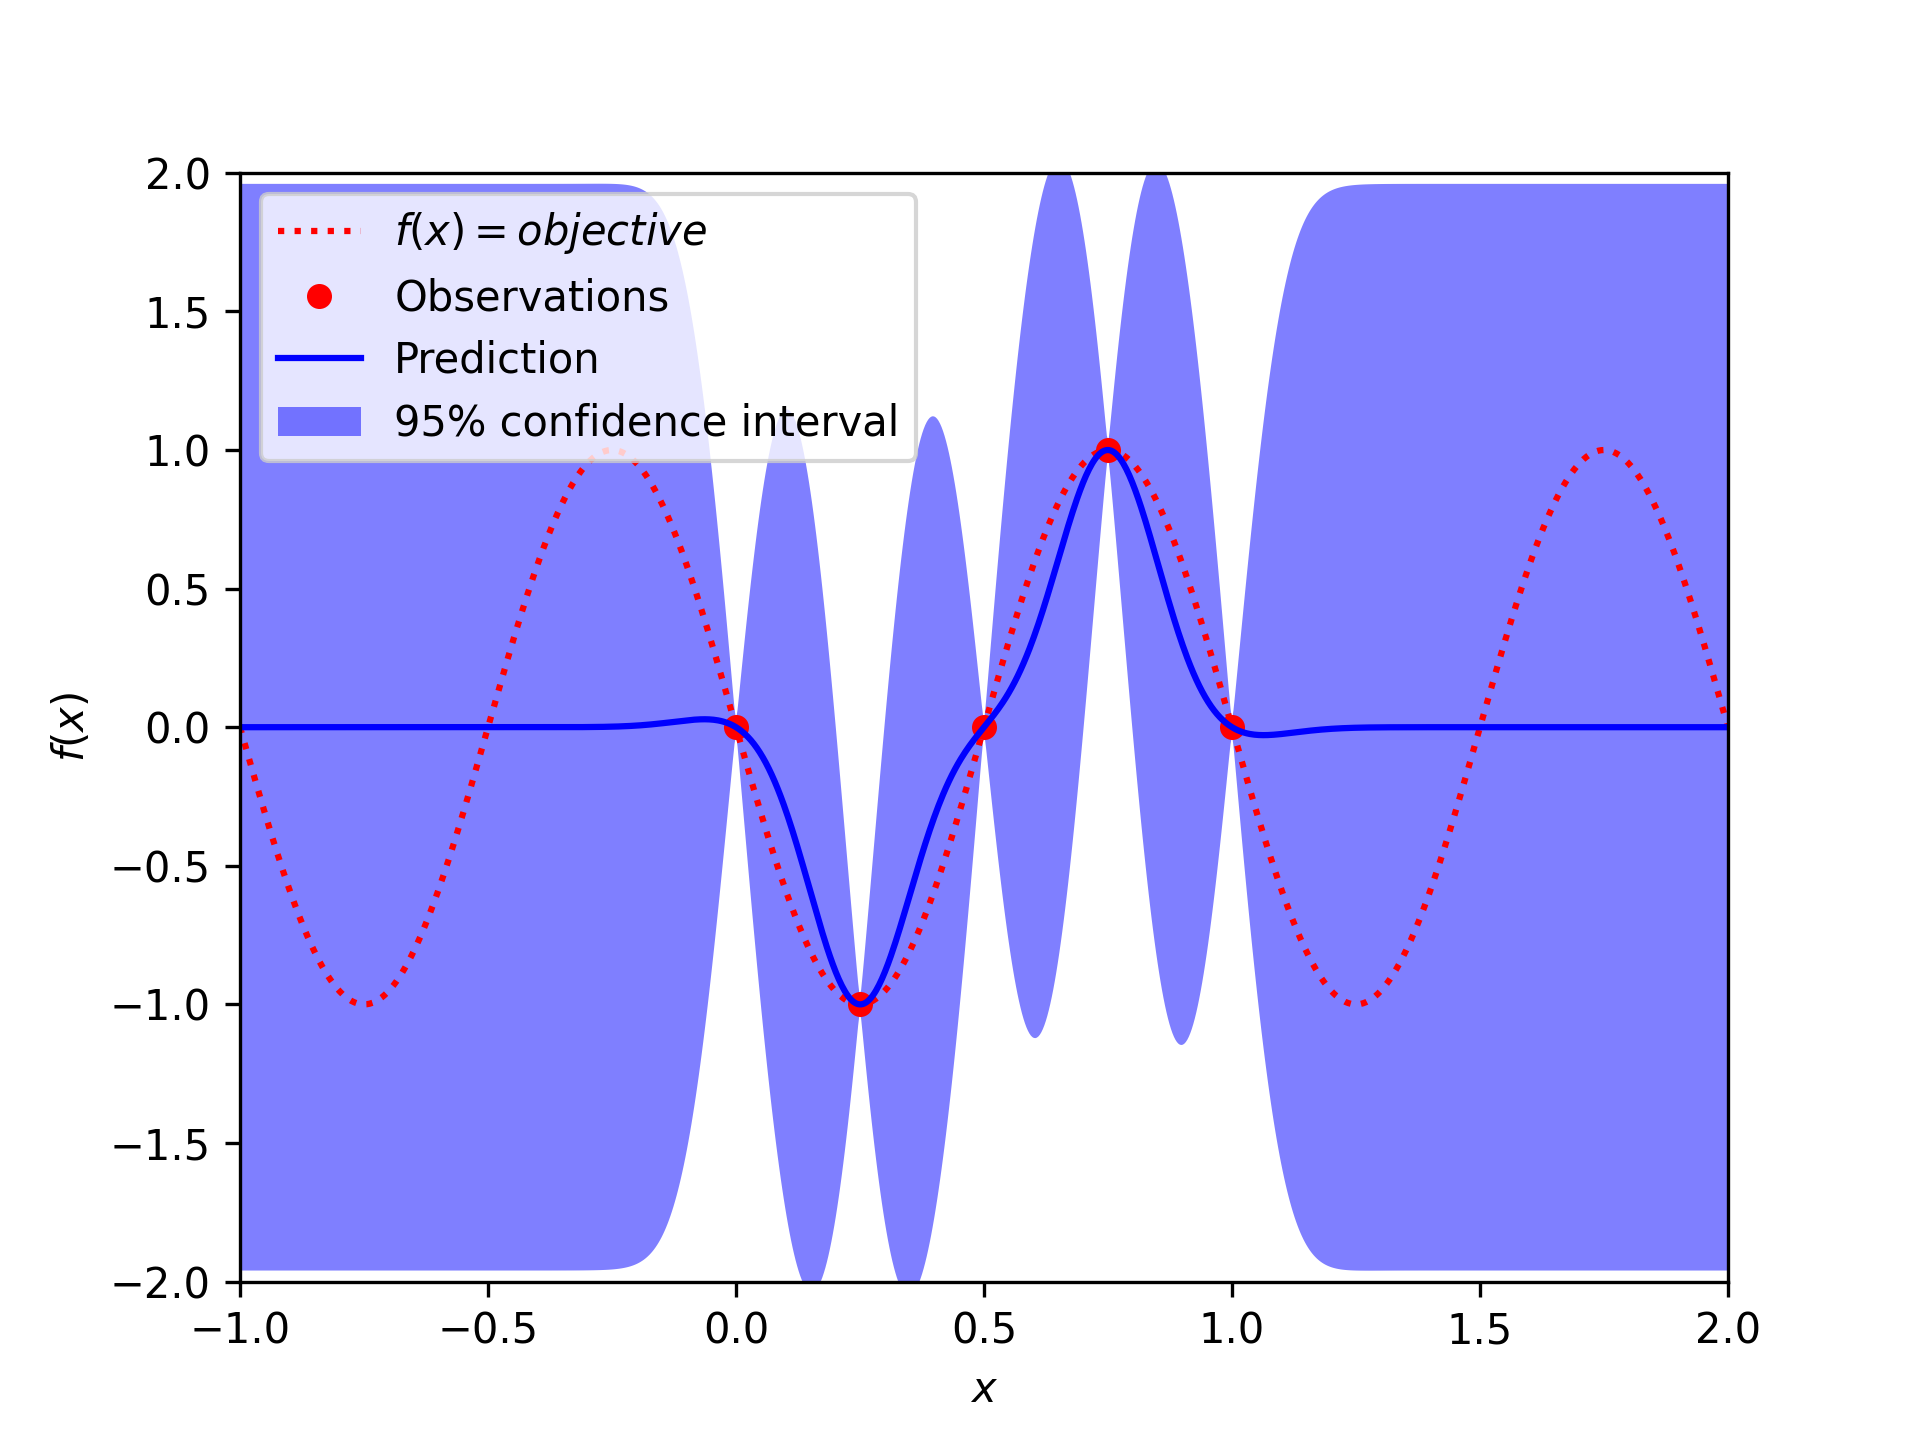
\includegraphics[width=0.75\linewidth]{regression_results2}
    \caption{
     Regression results for all three approaches for an objective function that is a sine wave. Here the wavelength set to 1, length scale set to 0.1, noise parameter set to 0.01, with 1000 basis centers spread across a domain from -5 to 5, and 5 training data points spread equidistantly over a domain from 0 to 1. The mean is presented with a blue line, and two standard deviations of the prediction uncertainty in the blue area, with the training data and objective in red. Since the length scale is now smaller than the distance between training data points, we see that the prediction uncertainty billows out between them. This figure was created with the associated code on Github.}
    \label{fig:example_regression2}
    \end{center}
\end{figure}

\section{Equating the Bayesian linear regression with the Gaussian process for a squared-exponential kernel}

We aim to find set of basis functions that relate to the Gaussian process prior kernel according to 
\begin{equation}
\label{define_K}
\begin{split}
     k_\text{GP}(\mathbf{x},\mathbf{x}') &= \sigma_0^2\phi^\top(\mathbf{x})\phi(\mathbf{x}) \\& = \sigma_0^2\sum_{i=1}^{N_B}k_\text{BLR}(\mathbf{x},\mathbf{x}''_i)k_\text{BLR}(\mathbf{x'},\mathbf{x}''_i) \\
     \mathbf{K}=k_{\text{GP}}(\mathbf{X},\mathbf{X})& = \sigma_0^2\boldsymbol{\Phi}^\top \boldsymbol{\Phi} + \sigma^2\mathbf{I}_N
     \end{split}
\end{equation}
where $N_B$ is the number of basis dimensions, our kernel bases are normalized so that $\boldsymbol{\phi}^\top\boldsymbol{\phi}=1$, and the desired prediction standard deviation far from the training data, but without any additional noise $\sigma$, is defined as $\sigma_0$. 

By Equation \ref{GP_posterior}, varying $\sigma_0$ changes our prediction covariance but not our prediction means. Note that while Equation \ref{define_K} resembles Equation \ref{eq:define_S}, the definition for $\mathbf{K}$ uses the inner product, while the definition of $\mathbf{S}$ uses the outer product.  Also, most definitions of the Gaussian process set $\sigma_0\rightarrow 1$, which is usually justified by scaling the training data so that the empirical standard deviation of our targets, $\sigma_\mathbf{y}$, also goes 1 and therefore $\sigma_0=\sigma_\mathbf{y}$, but the truth is that the scale can be arbitrarily chosen. We include the distinction here to help with the equivalence with BLR shortly. For now, what our choice of kernel shows is that if we scale our training targets, and expect $\sigma_0$ to scale accordingly so that $\sigma_0\propto\sigma_\mathbf{y}$, then it is the ratio $\frac{\sigma}{\sigma_\mathbf{y}}$ that defines the relative noise of our kernel.

According to the reproducing kernel Hilbert space (RKHS) theory, there is one set of $\psi$ that will accomplish this goal, but what is it? We consider the common case of 
\begin{equation}
\label{kernel}
    k_\text{GP}(\mathbf{x},\mathbf{x}') = \sigma_0^2\exp\left(\frac{(\mathbf{x}'-\mathbf{x})^2}{2l^2}\right) + \sigma^2 \delta(\mathbf{x}, \mathbf{x}')
\end{equation}which is a squared-exponential kernel with white noise added for the variation we expect in repeated measurements at the same point. Note that $l$ defines a length scale for the kernel.

Using the identity 
\begin{equation}
\label{gaussian_integral_identity}
    \int_{-\infty}^{\infty}e^{-a x^2 + b x + c}dx = \sqrt{\frac{\pi}{a}}e^{\frac{b^2}{4a}+c}
\end{equation}
we observe that 
\begin{equation}
\label{eq:gaussian_integral}
    \int_{-\infty}^{\infty}\exp\left(\frac{(x_0-x''_0)^2)}{2l^2}\right)\exp\left(\frac{(x'_0-x''_0)^2)}{2l^2}\right)dx''\propto\exp\left(\frac{x_0-x'_0}{4l^2}\right)
\end{equation}That is, if we perform an inner product over all possible $\mathbf{x}''$s for a basis function defined by a kernel with length scale $l$ at points $\mathbf{x}$ and $\mathbf{x}'$, this is equivalent to computing a different kernel between $x$ and $\mathbf{x}''$. To create a basis function set that will return a Gaussian kernel with length scale $l$, the kernel we use to generate that basis function set has the same form but with a length scale proportional to  $l/\sqrt{2}$.

Looking back at Equations \ref{BLR_posterior} and \ref{GP_posterior}, we can make the following correspondences for the means
\begin{equation}
    \overline{\mathbf{y}}_\ast\leftrightarrow\sigma^{-2}\boldsymbol{\phi}_\ast \boldsymbol{\Sigma} \boldsymbol{\Phi}^\top \mathbf{y} \leftrightarrow \mathbf{K}_\ast^\top \mathbf{K}^{-1} \mathbf{y}
\end{equation}
and the covariances
\begin{equation}
   \text{cov}(\mathbf{y}_\ast) \leftrightarrow \boldsymbol{\phi}_\ast\boldsymbol{\Sigma}\boldsymbol{\phi}_\ast^\top +\sigma^2 \mathbf{I}_{N_\ast}\leftrightarrow \mathbf{K}_{\ast\ast} - \mathbf{K}_\ast^\top \mathbf{K}^{-1} \mathbf{K}_\ast
\end{equation}.
The corresponding expressions certainly look similar, but there are noticeable differences. Moreover, they involve matrix multiplications on totally different dimensions: over the training data for GPs, but over the basis dimensions for BLRs. It begs the question, what if there were some kernel $k_\text{BLR}(\mathbf{x},\mathbf{x}')$ that could define a basis set 
\begin{equation}
\begin{split}
    \boldsymbol{\phi}(\mathbf{x})&=Z^{-1}(\mathbf{x})(k_\text{BLR}(\mathbf{x},\mathbf{x}_0),k_\text{BLR}(\mathbf{x},\mathbf{x}_1),\dots,k_\text{BLR}(\mathbf{x},\mathbf{x}_{N_B})) \end{split}
\end{equation}with normalization constant $Z(\mathbf{x})$ such that the above correspondences could become identities? We normalize according to
\begin{equation}
\label{eq:normalization}
\begin{split}
    Z(\mathbf{x}) &= \sqrt{\sum_{i=0}^{N_B}k_\text{BLR}(\mathbf{x},\mathbf{x}_i)^2} \\
    1 &= \boldsymbol{\phi}(\mathbf{x})^\top\boldsymbol{\phi}(\mathbf{x})
\end{split}
\end{equation}and by setting the prior covariance for the Bayesian linear regression proportional to the desired prediction standard deviation $\sigma_0$ far from the training data 
\begin{equation}
\label{eq:set_sigma_p_to_one}
\begin{split}
   \boldsymbol{\Sigma}_p=\sigma_0^2\mathbf{I}\\\sigma_p=\sigma_0
   \end{split}
\end{equation}we achieve the equivalence we've been looking for. In other words, we assume our prior weights have a mean of zero, are uncorrelated, and have a spread in their means equal to $\sigma_0$ far from the training data regardless of $k_\text{BLR}$, since the basis functions $\boldsymbol{\phi}(\mathbf{x})$ are normalized by Equation \ref{eq:normalization}. 

We can deepen our intuition behind the prior noise parameter by first observing that close to the training data our prediction variances are close to zero, but far from the training data, the variance is equal to $\sigma_0^2+\sigma^2$. To show this for the Gaussian process, we observe that $\mathbf{K}_0\rightarrow 0$ so that
\begin{equation}
\begin{split}
     \text{cov}(\mathbf{y}_0) &=\mathbf{K}_{00} - \mathbf{K}_0^\top \mathbf{K}^{-1} \mathbf{K}_0 \\
     &\rightarrow\mathbf{K}_{00} = \sigma_0^2+\sigma^2
     \end{split}
\end{equation}
To show this for the BLR, we start $\boldsymbol{\phi}_\ast^\top\boldsymbol{\Phi}\approx 0$ far from the training data. Due to the Woodbury matrix identity, we can derive
\begin{equation}
    \left(I + UV \right)^{-1} = I -U \left(I + VU \right)^{-1} V
\end{equation}so that when we look far from the training data, the prediction covariance is
\begin{equation}
\begin{split}
\text{cov}(\mathbf{y}_0)&=\boldsymbol{\phi}_0^\top\boldsymbol{\Sigma}\boldsymbol{\phi}_0 + \sigma^2  \\ 
&=  \sigma^2\left( \boldsymbol{\phi}_0^\top\left(\frac{\sigma^2}{\sigma_p^2}\mathbf{I}_{N_B}+\boldsymbol{\Phi}\boldsymbol{\Phi}^\top\right)^{-1}\boldsymbol{\phi}_0+1\right) \\
&= \sigma^2\left( \frac{\sigma_p^2}{\sigma^2}\boldsymbol{\phi}_0^\top\left(\mathbf{I}_{N_B}+\frac{\sigma_p^2}{\sigma^2}\boldsymbol{\Phi}\boldsymbol{\Phi}^\top\right)^{-1}\boldsymbol{\phi}_0+1\right) \\
&= \sigma^2\left( \frac{\sigma_p^2}{\sigma^2}\boldsymbol{\phi}_0^\top\left(\mathbf{I}_{N_B}-\frac{\sigma_p^2}{\sigma^2}\boldsymbol{\Phi}\left(\mathbf{I}_{N_B}+\frac{\sigma_p^2}{\sigma^2}\boldsymbol{\Phi}\boldsymbol{\Phi}^\top\right)^{-1}\boldsymbol{\Phi}^\top\right)\boldsymbol{\phi}_0+1\right) \\
&= \sigma_p^2\boldsymbol{\phi}_0^\top\boldsymbol{\phi}_0 + \sigma^2 -\frac{\sigma_p^4}{\sigma^2}\boldsymbol{\phi}_0^\top\boldsymbol{\Phi}\left(\mathbf{I}_{N_B}+\frac{\sigma_p^2}{\sigma^2}\boldsymbol{\Phi}\boldsymbol{\Phi}^\top\right)^{-1}\boldsymbol{\Phi}^\top\boldsymbol{\phi}_0 \\
&\approx\sigma_p^2\boldsymbol{\phi}_0^\top\boldsymbol{\phi}_0 + \sigma^2
\end{split}
\end{equation} 
By Equations \ref{eq:set_sigma_p_to_one} and \ref{eq:normalization}, we obtain 
\begin{equation}
\text{cov}(\mathbf{y}_0)\approx\sigma_0^2 + \sigma^2
\end{equation}In other words, the prior noise parameter determines the prediction variance far from our training data, since it determines the spread of our weights, multiplied by normalized basis functions, when they are not perturbed by our training data. Note that because of the basis normalization and our priors, if we include multiple kernels, for example a different length scale for each input dimension in a model that sums their weighted contributions rather than multiplies them, their concatenated basis functions need to be normalized by Equation \ref{eq:normalization}, rather than each kernel being normalized independently. 

If we mix kernel features with non-kernel features (e.g., linear, polynomial, etc.) in one model, we may normalize the kernels together, set the prior noise parameter for the kernel features to $\sigma_\mathbf{y}$, and set the L2 regularization constant to a predefined constant for the remaining features. In such a model, the normalized kernel features contribute a maximum prediction variance equal to the desired variance of our targets far from the training data, while the non-kernel features may contribute a prediction variance that far exceeds this value outside the domain of our training data, just as happens with standard Bayesian linear regression. Alternatively, one may apply an automatic relevance detection (ARD) regression and learn the effective prior noise parameters for each feature independently. However, a substantial drawback of ARD regression is that it doesn't have guarantees on convergence and is prone to underfitting, which is also why there may be challenges putting automatic tuning of $\sigma_p$ into production. We can, however,  learn $\sigma$ reliably using a sample of our training data, and we can learn $\sigma_p$ or $\lambda$ with cross-validation or other function minimization procedures.

Finally, we honor Equation \ref{eq:gaussian_integral} by setting
\begin{equation}
    k_\text{BLR}(x_0,x'_0)=\exp\left(\frac{x_0-x'_0}{4l^2}\right)
\end{equation}and we arrive at a Bayesian linear regression that produces the same predictions as the Gaussian process regression with kernel
\begin{equation}
    k_\text{GP}(x_0,x'_0)=\exp\left(\frac{x_0-x'_0}{2l^2}\right)
\end{equation} due to the normalization in Equation \ref{eq:normalization}.

Note that in this case, the posterior covariance isn't proportional to $k_\text{GP}$ for the same reason that it isn't proportional to $K_{\ast\ast}$ in Equation \ref{GP_posterior} or $\Sigma_p^{-1}$ in Equation \ref{BLR_posterior}. Rather, if we describe the posterior covariance as a pure kernel function, it would look something like 
\begin{equation}
    \text{cov}(\mathbf{y_\ast})= k_\text{post.}(\mathbf{x}_\ast,\mathbf{x}_\ast) =
    k_\text{equiv.}(\mathbf{x}_\ast,\mathbf{x}) k_\text{equiv.}^\top(\mathbf{x}_\ast,\mathbf{x})
\end{equation}\begin{equation}
\label{equivalen_kernel}
    k_\text{equiv.} = C\sigma\boldsymbol{\Sigma}^{1/2}k_\text{BLR}^\top(\mathbf{x}_\ast,\mathbf{x})
\end{equation}which means that inference on the posterior mixes up the basis functions defined by $k_\text{BLR}$ according to the operator $\boldsymbol{\Sigma}^{1/2}$, which is defined by performing a summation over the training points (just like with a Gaussian process).  For examples of this basis function set, see Figure \ref{fig:basis_large_width}.

What's a little weird about this equation is that it implies our covariance matrix would see its exponents divide by two due to the square root, but because of the identity of integrating over the product of two Gaussians in Equation \ref{gaussian_integral_identity}, it actually multiplies by two. Similarly, in Section \ref{sec:hyperparameter_tuning}, the derivation for computing the log marginal likelihood of the BLR (Equation \ref{eq:log_likelihood_BLR}) requires integrating over the product of two multivariate norms. The result inverts its proportionality with the determinant of the covariance matrix compared to either of the original multivariate norms.

\section{Equating the Bayesian linear regression with the Gaussian process for arbitrary kernels}

The previous section covered how to accomplish the equivalence between the Bayesian linear regression and the Gaussian process for a squared-exponential kernel for the GP. One take-away was that the equivalent basis in the BLR has a different length scale and prefactor, but since we can just normalize out prefactors, all that matters is the difference in length scales between the two formulations. The other main take-away is that we can use any arbitrary combination of our basis set and the BLR will learn new coefficients to account for that transformation, as evidenced in Equation \ref{equivalen_kernel}.

The drawback with the previous approach was that, while intuitive, it leaves us in the dark for performing this equivalence for arbitrary kernels. However, we can use the fact that we can use any linear combination of basis functions to achieve the same result. If that's the case, then let's eschew the manual integration and instead define our basis as the eigenvectors of the kernel used in the GP evaluated at the same basis centers used in the previous analysis.

We first calculate our eigenvectors (rows of $V$) and eigenvalues (diagonal elements of $D$) of the kernel without the noise parameter for an arbitrary set of points in the independent space $X'$ as follows:
\begin{equation}
 \mathbf{VDV}^\top=k_\text{GP}(\mathbf{X}',\mathbf{X}')-\sigma^2 \mathbf{I}=\mathbf{K}'-\sigma^2 \mathbf{I}_{N'}
\end{equation}giving us\begin{equation}
\begin{split}
\label{VDV}
    &\mathbf{VDV}^\top+\sigma^2 \mathbf{I} \\&= 
    \begin{bmatrix}
    k_\text{GP}(\mathbf{x}_0,\mathbf{x}_0) && k_\text{GP}(\mathbf{x}_0,\mathbf{x}_1) && \dots && k_\text{GP}(\mathbf{x}_0,\mathbf{x}_{N_B}) \\
    k_\text{GP}(\mathbf{x}_1,\mathbf{x}_0) && k_\text{GP}(\mathbf{x}_1,\mathbf{x}_1) && \dots && k_\text{GP}(\mathbf{x}_1,\mathbf{x}_{N_B}) \\
    \vdots && \vdots && \ddots && \vdots \\
    k_\text{GP}(\mathbf{x}_{N_B},\mathbf{x}_0) && k_\text{GP}(\mathbf{x}_{N_B},\mathbf{x}_1) && \dots && k_\text{GP}(\mathbf{x}_{N_B},\mathbf{x}_{N_B}) \\
    \end{bmatrix}
    \end{split}
\end{equation}

Note that previous equations look for the eigendecomposition of the kernel evaluated at an arbitrary set of points in independent space, omitting the white noise (diagonal entries in matrix form) but keeping the radial basis function (a Gaussian in this case) as well as the mean function $m(\mathbf{x})$ or $\mathbf{m}(\mathbf{X})$. The solution presented in this section works from these eigenvectors. To obtain a non-zero (mean) prediction far away from the data, we can either add subtract off the mean and add it back in during prediction, fit the intercept as a fixed hyperparameter, or concatenate a constant (usually 1) to the feature vectors $\boldsymbol{\phi}(\mathbf{x})$ and otherwise fit as normal. By comparison, GP practitioners either subtract off the mean or fit the mean through a constant added to every pair of points in the kernel (see Section \ref{sec:hyperparameter_tuning}. In both cases, adding the mean prediction increases the prediction variance at each point, in the BLR case due to the variance in the intercept term, and in the GP through the constant added to the kernel.

\begin{figure}
    \begin{center}
    \includegraphics[width=0.75\linewidth]{manualbasis_large_width}
    \includegraphics[width=0.75\linewidth]{eigenbasis_large_width}
    \caption{Top: The manual basis functions, which are length-scale-adjusted Gaussian distributions, centered at 0\%, 10\%, 20\%, and 30\% along the domain. Bottom: The eigenbasis functions $V$ for the largest four eigenvalues. Note that the sign of each function is arbitrary (can be flipped over the x-axis), and that these functions resemble the harmonic modes for an equivalent one-dimensional thick string with fixed endpoints one length scale outside the domain of our basis centers (off-plot).}
    \label{fig:basis_large_width}
    \end{center}
\end{figure}

\begin{figure}
    \begin{center}
    \includegraphics[width=0.75\linewidth]{manualbasis_small_width}
    \includegraphics[width=0.75\linewidth]{eigenbasis_small_width}
    \caption{Same as Figure \ref{fig:basis_large_width}, but for a kernel with a length scale $1/10^{\text{th}}$ the size. We see that the fixed endpoints of the hypothetical string are now right at the end of the basis center domain since the length scale of the kernel is so small.}
    \label{fig:basis_small_width}
    \end{center}
\end{figure}

To project our observations into this space, we convolve them with an normalized infinitesimal-width Gaussian kernel, that is, a dirac delta function $\delta$, but for computational purposes we choose a finite width that is equivalent to the distance between adjacent points in our sampling of the independent space $\mathbf{X}'$. While the choice is arbitrary, it makes sense to reuse the centers  to generate our basis set, that is, to set $\mathbf{X}'=(\mathbf{x}_0,\mathbf{x}_1,\dots,\mathbf{x}_{N_B})$.

We thus perform this projections as follows: 

\begin{equation}
    \mathbf{X}_\delta =
    \begin{bmatrix}
    \delta(\mathbf{x}_0,\mathbf{x}_0) && \delta(\mathbf{x}_0,\mathbf{x}_1) && \dots && \delta(\mathbf{x}_0,\mathbf{x}_{N_B}) \\
    \delta(\mathbf{x}_1,\mathbf{x}_0) && \delta(\mathbf{x}_1,\mathbf{x}_1) && \dots && \delta(\mathbf{x}_1,\mathbf{x}_{N_B}) \\
    \vdots && \vdots && \ddots && \vdots \\
    \delta(\mathbf{x}_{N},\mathbf{x}_0) && \delta(\mathbf{x}_{N},\mathbf{x}_1) && \dots && \delta(\mathbf{x}_{N},\mathbf{x}_{N_B}) \\
    \end{bmatrix}
\end{equation}
and then project onto the eigenbasis:
\begin{equation}
\begin{split}
    \boldsymbol{\Phi} &= \mathbf{X}_\delta \sqrt{\mathbf{D}}\mathbf{V}\\ \boldsymbol{\Phi} \boldsymbol{\Phi}^\top&=\mathbf{VDV}^\top\\&=\mathbf{K}'-\sigma^2 \mathbf{I}_{N'}
    \end{split}
\end{equation}
and similarly for our test data points at $\mathbf{X}_\ast$. We then perform the same procedure as for Bayesian linear regression (Equation \ref{BLR_posterior}). For examples of this basis function set, see Figure \ref{fig:basis_large_width}.


What happens to the eigenbasis when we change the width of the kernel? For small length scales (see Figure \ref{fig:basis_small_width}), the eigenbasis resembles the vibrational modes of a string (in one dimension, a plane in two dimensions, etc.) bounded by the domain of the basis centers, as if the string is perfectly fixed at its endpoints like on a guitar. As the length scale grows larger, as in Figure \ref{fig:basis_large_width}, we see that the eigenbases actually taper to the edges of the basis center domain with a length scale proportional to the one used for the kernel. The best possible approximation extends the domain of basis centers to plus and minus infinity, and when we take this approach in our calculations, we find that the same intuition applies but the interpretation changes slightly. The eigenbases with the highest eigenvalues resemble sine-waves in the training data domain and the wavelengths of adjacent eigenbases increment proportionally to the kernel wavelength. Similarly, the Taylor expansion of a Gaussian involves sine and cosine waves of differing wavelengths whose differences are proportional to the Gaussian length scale.

There is meaning held in the eigenvalues $\text{diag}(\mathbf{D})$. If we look at the eigenvalues for the linear system \begin{equation}\left(\sigma_p^{-2}\boldsymbol{\Phi}\boldsymbol{\Phi}^\top\right)\mathbf{u}_i=\mathbf{u}_i\end{equation} defined by $(\lambda_1,\lambda_2,\dots,\lambda_N)=\sigma_p^{-2}\text{diag}(\mathbf{D})$, by Section 3.5.3 of \cite{bishop}, we see that the quantity
\begin{equation}
\label{eq:gamma}
\gamma=\sum_{i=1}^{N}\frac{\lambda_i}{\sigma_p^{-2} + \lambda_i}
\end{equation} defines the effective number of parameters by which we can alter our noise parameter \begin{equation}\sigma_\text{unbaised}=\sigma\frac{N}{N-\gamma}\end{equation} to get the unbaised covariance matrix \begin{equation}\boldsymbol{\Sigma}_\text{unbaised}^{-1}=\sigma_\text{unbiased}^{-2}\boldsymbol{\Phi}\boldsymbol{\Phi}^\top+\boldsymbol{\Sigma}_p^{-1}\end{equation} of our model parameters $\boldsymbol{\theta}$. 

Note that whether we use the biased or unbiased noise parameter and covariance matrix does not affect our mean predictions, as shown in Equations \ref{eq:define_S} through \ref{BLR_posterior} , at least from the perspective where the regularization constant defined in Equation \ref{eq:lambda} is kept constant (not to be confused with the eigenvalues  $\lambda_i$). Also note that Equation \ref{eq:gamma} establishes an implicit solution for $\sigma_p$ which can be used to maximize the marginal likelihood over $\sigma_p$ through iteration if we don't set it to $\sigma_\mathbf{y}$, although instabilities arise if the iterations for both $\sigma_p$ and $\sigma$ run concurrently, causing the uninformative result $\sigma_p\rightarrow 0$, $\sigma \rightarrow \sigma_\mathbf{y}$, and $\overline{\boldsymbol{\theta}} \rightarrow \mathbf{0}$. 

When \cite{bishop} examines Equation {eq:gamma}, the text is mostly interested in how $\gamma$ alters with $\sigma_p$ by way of the regularization constant $\lambda$. However, we fix $\sigma_p=\sigma_\mathbf{y}$ when equating BLR with GP so we are more interested in how $\gamma$ alters with our other model hyperparameters. Given the same set of training data of $N$ rows, we find that we can cause $\gamma$ to asymptotically approach $N$ with two changes: increase the number of basis functions (centers of Gaussian distributions), and/or decrease the noise parameter $\sigma$. In other words, both changes to the problem increase the ability and need of the model to resolve more information than can be offered by just a few (well-chosen) basis functions. In the regime of many data points and fewer basis functions, $\gamma$ will asymptotically approach the number of basis functions as we increase $\sigma$.

We can perform a couple of simplifications to the procedure outlined in this section by considering two ways to reduce the computational complexity: (1) reduce the number of basis centers so that they are spaced according to the length scales of the original kernel and (2) reduce the number of eigenvectors (by filtering out those with small eigenvalues). The first works well, except when the variation in the training set y-values is greater than can be afforded by the length scale of the kernel. A GP or equivalent BLR will fit more closely to these widely-varying observations than one with a sparser basis set. 

Similarly, the second approach loses spatial resolution in proportion to how many eigenvectors are discarded, and in our experience, we found this approach to be very prone to meaningfully changing your calculations. Note that just as is the case with the manually-derived basis functions, the BLR will only produce equivalent predictions within the domain that the basis functions are not infinitesimally small.

\section{Tuning the noise parameter and kernel hyperparameters in both formalisms}\label{sec:hyperparameter_tuning}

There are only a few models in common circulation that allow you to learn the parameters using explicit and deterministic update rules. Of the two most prominent, well-studied, and easy-to-implement algorithms, one is the Bayesian linear regression with a fixed prior noise parameter or L2 regularization constant, and optionally with a fixed data noise parameter (the current discussion cover the case of fixed noise parameter, \cite{KoyoteScience} covers the learned case). The other is the Gaussian process, with a fixed data noise parameter, as discussed in this document. As we have covered, both are actually parts of the same continuum between high featurization and large amounts of data.  The secret ingredient for these models is that due to their assumptions, it is possible to analytically integrate the prediction 
\begin{equation}
    p_{\boldsymbol{\theta}}(\mathbf{y}_\ast|\mathbf{X}_\ast,\boldsymbol{\sigma}) = \int p(\mathbf{y}_\ast|\mathbf{X}_\ast,\boldsymbol{\theta})p(\boldsymbol{\theta}|\boldsymbol{\sigma})d\boldsymbol{\theta}
\end{equation}when $p(\mathbf{y}_\ast|\mathbf{X}_\ast,\boldsymbol{\theta})$ is defined by a multivariate norm centered on a function defining the mean (and mode) and another function defining the covariance. Here, we represent the hyperparameters of the model by the vector of noise parameters $\boldsymbol{\sigma}$ which could include $\sigma$, $\sigma_p$, or both. In fact, the hyperparameters could also include the lengths scales of our kernel or basis functions, and even individual prior noise parameters for each data point. Note that the model parameters $\boldsymbol{\theta}$ are defined by the measured function values $\mathbf{f}(\mathbf{X})$ for the Gaussian process, while in the Bayesian linear regression they are the coefficients of the basis functions.  

Alternatively, many models for which the prediction integral is intractable simply perform one prediction at the set of parameters $\boldsymbol{\theta}$ at the maximum a posteriori (MAP) when there is a prior $p(\boldsymbol{\theta})$, or the maximum likelihood estimate (MLE) when there is no prior or it is uniform and uninformative. In the Laplace approximation, which treats all models like they were Bayesian linear regressions, the spread in the probability mass for the model parameters around the MAP or MLE is modeled as a multivariate Gaussian whose covariance matrix is related to the Fisher information matrix, allowing us to compute a tractable prediction integral again.

The posterior distribution for our targets is provided by  \begin{equation} p(\mathbf{y}|\mathbf{X}, \boldsymbol{\theta})=\frac{p(\boldsymbol{\theta}|\mathbf{X},\mathbf{y})p(\mathbf{y})}{p_\mathbf{y}(\boldsymbol{\theta}|\mathbf{X})}\end{equation}or equivalently \begin{equation} p(\mathbf{y}|\mathbf{X}, \boldsymbol{\theta},\boldsymbol{\sigma})=\frac{p(\boldsymbol{\theta}|\mathbf{X},\mathbf{y},\boldsymbol{\sigma})p(\mathbf{y}|\boldsymbol{\sigma})}{p_\mathbf{y}(\boldsymbol{\theta}|\mathbf{X},\boldsymbol{\sigma})}\end{equation}and the inverse relationship is
\begin{equation}    p(\boldsymbol{\theta}|\mathbf{X},\mathbf{y},\boldsymbol{\sigma})=\frac{p(\mathbf{y}|\mathbf{X},\boldsymbol{\theta},\boldsymbol{\sigma})p(\boldsymbol{\theta}|\boldsymbol{\sigma})}{p_{\boldsymbol{\theta}}(\mathbf{y}|\mathbf{X},\boldsymbol{\sigma})}
\end{equation}where
\begin{equation}
\label{eq:define_marginal_likelihood}
  p_{\boldsymbol{\theta}}(\mathbf{y}|\mathbf{X},\boldsymbol{\sigma})=\int p(\mathbf{y}|\mathbf{X},\boldsymbol{\theta})p(\boldsymbol{\theta}|\boldsymbol{\sigma})d\boldsymbol{\theta}
\end{equation}is the normalization factor, marginal likelihood, or the model evidence from Bayes' theorem (posterior = likelihood $\times$ prior / evidence). Since we are usually interested in maximizing the posterior with respect to $\mathbf{y}$ or $\boldsymbol{\theta}$, we usually ignore the denominators in the above equations, unless we decide to also optimize our hyperparameters, which we will now discuss.

We can consider this model to be hierarchical -- first we set the model hyperparameters $\boldsymbol{\sigma}$, giving us our prior distribution  over the model parameters $\boldsymbol{\theta}$, and then we compute our posteriors. While we expect our model to learn its parameters, we may also want a model to learn the hyperparameters. This requires us to go up one level in the hierarchy, where we look at the posterior distribution of our hyperparameters

\begin{equation}
\label{eq:posterior_sigma}
    p_{\boldsymbol{\theta}}(\boldsymbol{\sigma}|\mathbf{X},\mathbf{y})=\frac{p_\boldsymbol{\theta}(\mathbf{y}|\mathbf{X},\boldsymbol{\sigma})p(\boldsymbol{\sigma})}{p_{\boldsymbol{\sigma}}(\mathbf{y}|\mathbf{X})}
\end{equation}where
\begin{equation}
\label{eq:marginal_marginal_likelihood}
   p_{\boldsymbol{\sigma}}(\mathbf{y}|\mathbf{X})=\int p(\mathbf{y}|\mathbf{X},\boldsymbol{\sigma})p(\boldsymbol{\sigma})d\boldsymbol{\sigma}
\end{equation}and the inverse relationship (which we don't use) is 

\begin{equation}
    p_{\boldsymbol{\theta}}(\mathbf{y}|\mathbf{X},\boldsymbol{\sigma})=\frac{p_\boldsymbol{\theta}(\boldsymbol{\sigma}|\mathbf{X},\mathbf{y})p(\mathbf{y})}{p_{\mathbf{y}}(\boldsymbol{\sigma}|\mathbf{X})}
\end{equation}
That is, the MAP or MLE of the hyperparameters will occur when we maximize the marginal likelihood in Equation \ref{eq:define_marginal_likelihood}, which is also known as the evidence of the model itself when we integrate over the parameters.

The above discussion leaves you to wonder that, since there is uncertainty in your hyperparameters when we don't fix them in advance and instead fit them along with the model parameters, how their uncertainty would add to the uncertainty of your predictions. Since Equation \ref{eq:marginal_marginal_likelihood} is generally intractable, we use the Type-II maximum likelihood estimation, or empirical Bayes approximation, whereby we keep our hyperparameters fixed for several different guesses and then learn the MLE of the influenced parameters, and maximize with respect to the hyperparameters we explore over. If we are comfortable with using the MAP or MLE for our mean and the Laplace approximation (defining the spread in hyperparamters by the Fisher information matrix or local curvature), we can stop here. A well-thought out discussion of why we should be satisfied with this approximation can be found in \cite{MacKay99}.

Using Equation \ref{eq:posterior_sigma}, we can compare two models with hyperparameters $\boldsymbol{\sigma}_1$ and $\boldsymbol{\sigma}_2$, 
\begin{equation}\frac{p(\boldsymbol{\sigma}_1|\mathbf{X},\mathbf{y})}{p(\boldsymbol{\sigma}_2|\mathbf{X},\mathbf{y})}=\overbrace{\frac{p_{\boldsymbol{\theta}}(\mathbf{y}|\mathbf{X},\boldsymbol{\sigma}_1)}{p_{\boldsymbol{\theta}}(\mathbf{y}|\mathbf{X},\boldsymbol{\sigma}_2)}}^\text{Bayes' factor}\frac{p(\boldsymbol{\sigma}_1)}{p(\boldsymbol{\sigma}_2)}\end{equation}giving us Bayes' factors (used in the Bayesian information criterion, or BIC). This tells us that we can compare them using their marginal likelihoods without having to perform the nasty integrals from the denominator, assuming that the prior distributions of the hyperparameters are identical.

We compute the marginal likelihood by integrating the product of the multivariate normal likelihood distribution dependent on $\mathbf{X},\mathbf{y},\boldsymbol{\theta},\boldsymbol{\Sigma}, \sigma$, and the prior multivariate normal prior distribution of the parameters dependent on $\sigma_p$, over the model parameters $\boldsymbol{\theta}$. Meanwhile, the normalized multivariate distribution $\mathbf{y}|\mathbf{X} \sim \mathcal{N}(\mathbf{y}|\mathbf{m},\boldsymbol{\Sigma}_f)$ is given by
\begin{equation}
\begin{split}
    \mathcal{N}(\mathbf{y}|\mathbf{m},\boldsymbol{\Sigma}_f)& =\frac{1}{\sqrt{(2\pi)^N |\boldsymbol{\Sigma}_f|}} \exp \left(-\frac{1}{2}(\mathbf{y}-\mathbf{m})^\top\boldsymbol{\Sigma}_f^{-1}(\mathbf{y}-\mathbf{m})\right) \\
   \log p(\mathbf{y}|\mathbf{X})& = -\frac{1}{2}(\mathbf{y}-\mathbf{m})^\top\boldsymbol{\Sigma}_f^{-1}(\mathbf{y}-\mathbf{m})-\frac{1}{2}\log |\boldsymbol{\Sigma}_f|-\frac{N}{2}\log 2\pi
   \end{split}
\end{equation} We  thus express our marginal likelihood as
\begin{equation}
\begin{split}
    p_{\boldsymbol{\theta}}(\mathbf{y}|\mathbf{X},\boldsymbol{\sigma})&=\int p(\mathbf{y}|\mathbf{X},\boldsymbol{\theta})p(\boldsymbol{\theta}|\boldsymbol{\sigma})d\boldsymbol{\theta} \\
    &= \int \mathcal{N}(\mathbf{y}|\boldsymbol{\Phi}\boldsymbol{\theta},\sigma^2\mathbf{I}_N)\mathcal{N}(\boldsymbol{\theta}|\mathbf{0}_{N_B},\sigma^2\mathbf{I}_{N_B})d\boldsymbol{\theta}
    \end{split}
\end{equation}After completing the squares on the two squared exponentials and normalizing\footnote{Similarly, you can evaluate the integral from Equation 3.77 using Equation 2.115 in Exercise 3.16 from \cite{bishop}. Bishop's book doesn't cover the derivation, but you can find solutions for Exercise 3.16 online. A detailed and satisfying derivation can be found at \href{ http://www.utstat.utoronto.ca/~radford/sta414.S11/week4a.pdf}{\texttt{http://www.utstat.utoronto.ca/~radford/sta414.S11/week4a.pdf}}}, we arrive a Equation 3.86 from \cite{bishop}: 
\begin{equation}
\label{eq:log_likelihood_BLR}
\begin{split}
    &\log p_{\boldsymbol{\theta}}(\mathbf{y}|\sigma_p, \sigma) \\=&- \frac{1}{2\sigma^2}\left(||\mathbf{y}-\boldsymbol{\Phi}\overline{\boldsymbol{\theta}}||^2 + \frac{\sigma^2}{\sigma_p^2}\overline{\boldsymbol{\theta}}^\top\overline{\boldsymbol{\theta}}\right) \\&-\frac{1}{2}\left( \log|\boldsymbol{\Sigma}^{-1}|+2 N \log \sigma +2N_B \log \sigma_p \right)\\&-\frac{N}{2}\log 2\pi
    \end{split}
\end{equation}Note that the data term $- \frac{1}{2\sigma^2}||\mathbf{y}-\boldsymbol{\Phi}\overline{\boldsymbol{\theta}}||^2 $ becomes a constant ($-\frac{1}{2}$) if we learn $\sigma$ from the residuals, and that we are expressing our solution in terms of the mean (learned) model parameters $\overline{\boldsymbol{\theta}}=\sigma^{-2}\boldsymbol{\Sigma}\boldsymbol{\Phi}^\top$ from Equation \ref{theta_distribution}.

For the Gaussian process, we also obtain the log marginal likelihood through integration over two Gaussians. In this case, however, we integrate over the measured input data $\mathbf{f}(\mathbf{X})$, instead of a set of explicit model parameters $\boldsymbol{\theta}$, so that
\begin{equation}
\begin{split}
    p_{\mathbf{f}}(\mathbf{y}|\mathbf{X},\boldsymbol{\sigma})&=\int p(\mathbf{y}|\mathbf{X},\mathbf{f})p(\mathbf{f}|\mathbf{X},\boldsymbol{\sigma})d\mathbf{f} \\
    &= \int \mathcal{N}(\mathbf{y}|\mathbf{f},\sigma^2\mathbf{I}_N)\mathcal{N}(\mathbf{f}|\mathbf{0}_{N},\mathbf{K}_\text{RBF})d\mathbf{f}
    \end{split}
\end{equation}Using the identity in Equation A.7 from \cite{rasmussen} with the values
\begin{equation}
\begin{split}
    \mathbf{a} &= \mathbf{f} \\
    \mathbf{A} &= \sigma^2\mathbf{I}_N \\
    \mathbf{b} &= \mathbf{0}_N \\
    \mathbf{B} &= \mathbf{K}_\text{RBF}
\end{split}
\end{equation}and noting that $\mathcal{N}(\mathbf{x}|\mathbf{y},\boldsymbol{\Sigma}_f)=\mathcal{N}(\mathbf{y}|\mathbf{x},\boldsymbol{\Sigma}_f)$, we arrive at Equations 2.30 and 5.8 in \cite{rasmussen}:
\begin{equation}
\label{eq:marginal_likelihood_of_GP}
\begin{split}
    \log p(\mathbf{y}|\mathbf{X},\mathbf{K}_\text{RBF}) =& -\frac{1}{2}\mathbf{y}^\top \mathbf{K}^{-1} \mathbf{y} \\&- \frac{1}{2}\log|\mathbf{K}|\\& - \frac{N}{2}\log 2\pi
    \end{split}
\end{equation}where the vertical bars represent the determinant operator and $\mathbf{K}=\sigma_0^2\mathbf{K}_\text{RBF}+\sigma^2 \mathbf{I}_N$. We can make $\overline{\mathbf{f}}$ non-zero by adding a constant between every pair of points to the kernel $\mathbf{K}_\text{RBF}$. Given these likelihoods, you can also optimize the noise parameter and length scales of the equivalent BLR the same way that is canon with GPs: you perform multiple gradient descents in the negative log marginal likelihood, since the landscape is pretty smooth, although not convex, and therefore may have multiple local minima. 

Diving in more deeply, we see that the first terms, which represent the data fit, are equivalent:
\begin{equation}
    \sigma^{-2}||\mathbf{y}-\overline{\boldsymbol{\theta}} ^\top \Phi ||^2 +\sigma_p^{-2} \overline{\boldsymbol{\theta}}^\top\overline{\boldsymbol{\theta}} = \mathbf{y}^\top \mathbf{K}^{-1} \mathbf{y} 
\end{equation}and at first it may seem surprising to include the regularization term proportional to $\overline{\boldsymbol{\theta}}^\top\overline{\boldsymbol{\theta}}$ in this equation. Keep in mind that the regularization term is enforced in the BLR by the prior with uncorrelated weights with a spread equivalent to a pre-defined noise parameter $\sigma_p$, and while the regularization is enforced in the GP by the prior kernel which includes the noise parameter in its white noise component, that is, it is the sum of the white noise kernel and the radial basis function kernel. 

The second terms, which represent model complexity, are also equivalent since \begin{equation}
\begin{split}
\frac{1}{\sigma^2}\mathbf{K}&= \mathbf{I}_N+\frac{\sigma^2_0}{\sigma^2}\boldsymbol{\Phi}^\top\boldsymbol{\Phi} \\
\sigma_p^2\boldsymbol{\Sigma}^{-1} &=\mathbf{I}_{N_B}+ \frac{\sigma_p^2}{\sigma^2}\boldsymbol{\Phi}\boldsymbol{\Phi}^\top
\end{split}\end{equation}By the identity $|\mathbf{I}_{N_\text{inner}}+\mathbf{UV}^\top|=|\mathbf{I}_{N_\text{outer}}+\mathbf{V}^\top\mathbf{U}|$ and by setting $\sigma_p=\sigma_0$ we obtain
\begin{equation}
|\boldsymbol{\Sigma}^{-1}|\sigma_p^{2N_B}=|\mathbf{K}|\sigma^{-2N}\end{equation}\begin{equation}
-\log|\boldsymbol{\Sigma}|+2N_B\log\sigma_p=\log|\mathbf{K}|+ 2N\log\sigma\end{equation}\begin{equation}
\log|\boldsymbol{\Sigma}^{-1}|+2N\log\sigma+2N_B \log \sigma_p=\log|\mathbf{K}|\end{equation}The third terms are trivially equivalent.

There are many ways to learn the noise parameter $\sigma$, in particular because it doesn't affect the other learned model parameters in a BLR except through regularization when $\sigma_p$ is fixed or learned. First, when inputs or basis functions are orthogonal (which is not the case for the Gaussian basis functions considered in this document), when the regularization constant is fixed, and during updates one-row-at-a-time, $\sigma$ can be learned using linear algebra identities according to Equation 3.73 in \cite{murphy}. Second, with either fixed $\lambda$ or $\sigma_p$, we can determine $\sigma$ empirically, using a randomized subset of the training data as an approximation if necessary. Lastly, in all cases, we can learn the noise parameter for the BLR by minimizing the negative log marginal likelihood, using a gradient descent method for example, just as we can learn the kernel hyperparameters in a GP. These methods work very well for single hyperparameters, but become less reliable for multiple ones, since they require multiple gradient descents and are prone to finding local minima rather than the global minimum.

For learning just $\lambda$ or $\sigma_p$ with fixed $\sigma$, there are several implicit (circular) solutions, such as the ones presented in Sections 3.5.2 and 9.3.4 from \cite{bishop}, but they require multiple iterations over the dataset. There is a silver lining, however. Online, incremental, or sequential versions of the BLR can update $\lambda$ or $\sigma_p$ at each step from an initial guess (usually taken to be close to zero) based on the observed or fixed $\sigma$ determined by the previous guess. Thus, the implicit solution is iterated over automatically as we add each new row of data. The drawback with this approach is that updating your BLR posteriors one row at a time is computationally inefficient compared to batch processing. On the other hand, there are many applications, such as contextual multi-armed bandits and hyperparameter tuning, where obtaining each row of data is time-intensive, so that incremental solutions are preferred. In these cases, feast on that free lunch all you want.

\printbibliography
\end{document}
